%\RequirePackage[l2tabu, orthodox]{nag}  %Checks for older packages

\documentclass[11pt,a4paper]{article}
% \documentclass[10pt]{extreport} $ allos to make the font smaller
\usepackage[utf8]{inputenc}

\usepackage{amsmath}
\usepackage{amsfonts}
\usepackage{indentfirst}
\usepackage{amssymb}
\usepackage[font={footnotesize}]{caption} %Makes the captions small

%\usepackage{algorithm}
%\usepackage{algpseudocode}
\usepackage[linesnumbered,ruled,vlined]{algorithm2e}

%% Figures packages
\usepackage[pdftex]{graphicx}
\usepackage{float}   %Es para colocar el objeto flotante exactamente donde se ponga el comando con H
\usepackage{caption}
\usepackage{subcaption}
\graphicspath{{../results/}}
\usepackage{sidecap}  %Para poner figuras a los lados


\usepackage{setspace} % Needed for Pyton syntax highlight
\usepackage{listings}    % Include the listings-package, nice verbatim for code
\usepackage{color}
\usepackage{courier}


\usepackage{cleveref} %puts figure and equation appropiately \cref{}

\usepackage{natbib} %For bibliography
%\usepackage{cite}
\usepackage{framed} % To use boxes, or frames around text

\usepackage{parskip} %Para saltos entre parrafos
\setlength{\parindent}{0pt}
\setlength{\parskip}{\baselineskip}
\usepackage[a4paper,margin=0.8in]{geometry}  %%Cambiar los margenes

\newcommand{\HRule}{\rule{\linewidth}{0.5mm}}
\newcommand{\Wb}{\mathbf{w}}

%\usepackage{hyperref} %This should be loade after most of the other packages
% \hypersetup{colorlinks=true}  %Para que los hiperlinks cuando se hagan referencias aparezcan en colores.



\definecolor{dkgreen}{rgb}{0,0.6,0}

\title{Lab12: DD2380 }
\author{
Ramon Heberto Martinez Mayorquin  hramon@kth.se
Akash Kumar Dhaka  akashd@kth.se
}



\begin{document}

\begin{titlepage}
\begin{center}
%\includegraphics[width=0.15\textwidth]{logo}\\[1cm]

\textsc{\LARGE Kungliga Tekniska högskolan}\\[1.0cm]

\textsc{\Large Summer School: Introduction to High Performance Computing}\\[2.0cm]



\begin{figure}[H]
	\centering
 
\includegraphics[width=0.35\textwidth]{Kth_logo.png}
\end{figure}
%\\[1cm]
%

% Title
\HRule \\[0.4cm]
{ \huge  Project: Stochastic Gradient Descent in CUDA.
}\\[0.4cm]
\HRule \\[1.5cm]

% Author and supervisor

Authors: Ram\'on  Mart\'inez, Theodoros Vasiloudis   \\
\large Professors: One Dude, The other dude.  \\ [2.5cm]
%\normalsize Presenta \\
%\large Supervisors 2: Jan Antolik \\[2.5cm]

\textsc{\Large School of Computer Science and Communication \\
PDC Center for High Performance Computing}\\ [1.0cm]
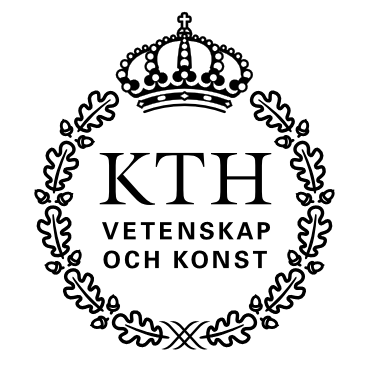
\includegraphics[width=0.15\textwidth]{KTH_black.png}\\[1.5cm] % Controls the distance till the new object
% Bottom of the page
{\large 15 September of 2015}

\end{center}
\end{titlepage}

\begin{abstract}
Parallelize this parallelize that.

\end{abstract}

\section{Stochastic Gradient Descent}

%TODO: (Throughout text) Ensure vectors are typed with \mathbf{v}, have \Wb command for w

One of the most common problems in estimation, optimization theory and machine learning is
minimizing an objective function \citep{bottou2010large}. Consider the \textit{loss} function $Q(z,
w)$. This function depends both on a sample $z=(x, y)$ which is a pair made of an input $x$ and an
output $y$ and on the vector $\Wb$ which parametrizes the function that connects the input to the
output. In such a context we would like to find the vector $\Wb$ that minimizes this error averaged
over our data. In a more mathematical parlance we write that following:

\begin{equation}
E(w) = \frac{1}{n} \sum_{i=1}^n Q(z_i, w)
\end{equation}

where $i$ the sample index, as we go through the complete dataset $\mathbf{z}$.

The Gradient Descent method proposes moving in the direction of the gradient in order to
find $w$. That is, we perform steps of a given size in the direction of the gradient of the loss function and update $w$ at every step:

\begin{equation}
w_{t + 1} = w_t - \gamma \sum_{i=1}^n \triangledown_w Q(z_i, w)
\end{equation}

where $\gamma$ controls the step size. This quantity is usually called the learning rate and
controls the speed or rate of change in $w$. $gamma$ is of crucial importance for the
convergence or divergence of the algorithm, setting $gamma$ too high leads to large changes at each iteration and
making it possible for the algorithm to diverge. If we set $gamma$ too small the algorithm
will not perform enough exploration, leading to slow convergence.

Under sufficient regularity assumptions when the initial estimate of $w$ is close enough to the
minimum and the learning rate is small enough this algorithm can achieve linear convergence
\citep{dennis1996numerical}.

Stochastic Gradient Descent (SGD) is a variation of the scheme proposed above that can be used
when the complete dataset is not available at runtime, e.g. in a streaming setting,
or when the data does not fit into memory.
In this case instead of taking the average gradient over the complete data we only use the local
gradient taken from a single datapoint to calculate the direction of movement:

\begin{equation}
w_{t + 1} = w_t - \gamma  \triangledown_w Q(z_i, w)
\end{equation}

It follows from the algorithm that this optimization can be implemented online due to the fact that
very little memory is needed for the calculation. The convergence of stochastic gradient descent is granted
in  some mild conditions when the learning rate $\gamma$ decreases over time in such a way that the
series  indexed by them does not diverge \citep{bottou2010large}.

In \citep{wilson2003general} it is shown, perhaps counter-intuitively, that batch gradient descent has
worse run-times and convergence characteristics when compared to stochastic gradient descent.

Mini-batch stochastic gradient descent lies somewhere in the middle between these two algorithms.
There, the optimization process is performed on small subsets of the complete dataset that are
called \textit{batches}. At each step in the algorithm we choose a random subset of the data,
calculate the gradient, and update the weights, based on the information we are able to get from
the batch. The main advantage in speed for mini-batch SGD comes from the fact that instead of the
matrix-vector multiplications that are necessary in plain SGD, we are able to batch samples
together and perform matrix-matrix multiplications, thereby allowing for a more efficient learning
process.

\section{Parallel Stochastic Gradient Descent}
\subsection{Related Work}

There exist a number of approaches for parallelizing SGD \citep{zinkevich2010parallelized,
recht2011hogwild, dekel2012optimal}, and each comes with some advantages and disadvantages. Some of
these algorithms are mostly intended to be used in a distributed setting, but can however be
adapted to function well in a highly parallel setting as well.

The approach presented in \citep{zinkevich2010parallelized} is an intuitive parallel extension of
SGD, where each processor solves a local SGD problem using a random partition of the
complete dataset, and the solutions from each processor are then communicated and averaged. This
approach involves practically no communication between the processors during the optimization
phase. While this is beneficial in terms of network/communication costs, it results in subpar
performance when it comes to the optimality of the solution.

\cite{recht2011hogwild} also propose an asynchronous algorithm which is aimed at problems with
sparse parameters, i.e. we assume that the cost function we are optimizing can be decomposed (to a
degree). This property makes it possible for individual processors to work on different parts of
$\Wb$, and perform gradient descent using only a single parameter from the complete weight vector,
making it possible to atomically update that single parameter, in parallel with the other
processors, without the need for locking the weight vector while one processor makes its updates.
While this approach allows for fast iterations since each processor can work and update his part of
the solution independently from the others, it has the additional assumption of problem sparsity
and the lack of communication between processors can often lead to diverging solutions
\citep{dai2015analysis}.

\cite{dekel2012optimal} show a distributed mini-batch SGD approach which they show is optimal in
terms of the \textit{optimality gap} which they define as the difference between the loss given by
the optimal weight vector $Q(z, w^*)$ and the approximation obtained by the algorithm, $Q(z,
\bar{w})$. The algorithm proposed uses mini-batches to calculate approximate gradients for each
processor, which are then summed and averaged across the different processors, and the averaged
gradient is used to update the weights at the end of each iteration. While this algorithm obviously
has higher communication costs when compared to the ones we described before, it can attain better
convergence guarantees, and enjoys faster convergence in terms of number of iterations, as the
different processors have access to more up-to-date and consistent sets of weights. One drawback of
this approach when it comes to highly parallel architectures however is that its parallelization
factor is limited by the minimum of number of batches and available processors.

\subsection{Algorithm Used}

For this work we chose a variant of the algorithm described by \cite{dekel2012optimal}, which involves the following steps:
%TODO: Write in algorithm format
\begin{enumerate}
	\item  	For each iteration:
	\begin{enumerate}
		\item Select a subset of the data of size $b$.
		\item Calculate the gradient for each data point in the batch.
		\item Sum and average the gradients for all data points in the batch.
		\item Update the weight vector according to the average gradient.
	\end{enumerate}
\end{enumerate}

We can write the above more formally in algorithmic form:

\begin{algorithm}
	\DontPrintSemicolon % Some LaTeX compilers require you to use \dontprintsemicolon instead
	\KwIn{A dataset $D$ of containing n $z=(x, y)$ items, initial learning rate $\alpha$}
	\KwOut{A vector of weights providing an approximate linear solution}
	Initialize $w$\;
	\For{$i \gets 1$ \textbf{to} $T$} {
		Select a random subset of $D$, $\mathbf{z}_s$\;
		\For(\textbf{parallel}){$j \gets 1$ \textbf{to} $b$} {
			$\hat{g_j} = \triangledown_w Q(z_j, w_i)$, where $z_j \in \mathbf{z}_s$\;
		}
		$\gamma = -(\alpha / \sqrt{i}))$\;
		Do parallel sum $\sum_j{\hat{g_j}}$ to compute the average gradient for the current batch, $\bar{g_i} = 1/j \sum_j{\hat{g_j}}$\;
		Do parallel scaling of the weight vector: $w_{i + 1} = w_i - \gamma \,  \bar{g_i}$\;

	}
	\Return{$w_T$}\;
	\caption{Mini-batch parallel SGD on a GPU}
	\label{algo:sgd-gpu}
\end{algorithm}

The difference of this algorithm when compared to the one by \cite{dekel2012optimal} is that where
they sum the gradients over all batches in order to reduce communication costs --the algorithm is
aimed at a distributed environment-- we are able to sum the gradient for the sample \textit{within}
each batch. We are able to do this due to the low communication costs that we have once all the
data is loaded to the GPU, and using this approach we able to tie the parallelization factor to the
size of the mini-batch $b$ instead of the number of batches $c$. Depending on the data size and
parameters, it usually true that $b \gg c$, allowing for better utilization of the GPU
architecture.

We employ parallelization then in 3 distinct parts of the algorithm: We calculate the gradients for
each sample in a batch in parallel, we sum the gradients in parallel through a transform/reduce
process, and scale the weight vector in parallel as well. The heaviest process computationally is
the gradient calculation.


\section{Implementation}
In this section we discuss the implementation tools and libraries that were used in the project.

\subsection{CUDA}
The CUDA platform was developed around 2009 \citep{nickolls2008scalable} and since then it has
allowed the research community to harness the power of GPU for computing processing and data
crunching without requiring expertise on graphical programming. The CUDA model is an extension of
ANSI C where certain operations are carried out in a thread basis on the GPU. In order to do so
CUDA provides a geometrical hierarchy that is composed of threads, blocks and grids. In this work
we have use CUDA through the Thrust library.

\subsection{Thrust}
Thrust is a parallel algorithms library aimed at increasing the productivity of programmers by
offering a model of programming similar to the one of the standard library on C++
\citep{bell2012thrust}. In other words this switches the attention from \textit{how} to compute
something to simply \textit{what} to compute. Among the most notorious features that
\textbf{Thrust} provides are parallel version of scan, sort and reduction which allow us to use
utilize those functions with arbitrary types and operations.

Furthermore Thrust provides a vector container with both host and device instances that allow us to demarcate where the operations are happening and takes care of the memory transfers.


\subsection{C+11}
Use of templates?

\section{Results}
In this section we will show results of our time measurements. In order to measure effectively we
use the CUDA functionality of events. The CUDA event API is the standard to bypass the non-blocking
nature of kernel calls. In our code we use a call to eventRecorder before and after the kernel and
then measure this difference. This is the time that we are going to be showing in our results from
now on.

\begin{tabular}{|c|c|c|}
\hline
Parameter & Description & Range \\
\hline
Batch Size & The size of the mini batch & • \\
\hline
Number of Samples & The number of training examples & • \\
\hline
Number of Features & The number of features of each training point & • \\
\hline
\end{tabular}

\section{Discussion}

\bibliographystyle{plainnat}
\bibliography{references}
\end{document}